\label{pt2:introduction}

\begin{figure}[t]
	\centering
	\begin{subfigure}{0.35\linewidth}
		\centering
		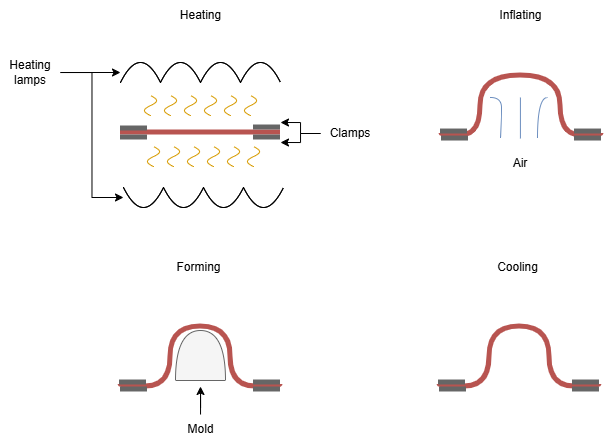
\includegraphics[width=\linewidth]{figures/thermoforming_process.png}
		\caption{The four stages of thermoforming}
		\label{fig:thermoforming_process}
	\end{subfigure}
	\hspace{0.1\linewidth}
	\begin{subfigure}{0.30\linewidth}
		\centering
		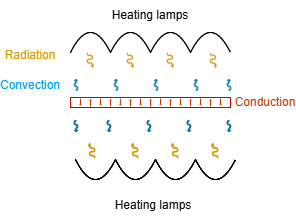
\includegraphics[width=\linewidth]{figures/raditaion_conduction_convection.png}
		\caption{Thermoforming heating phase: conduction, convection, and radiation}
		\label{fig:thermoforming_conduction_convection_radiation}
	\end{subfigure}
	
	\caption{Overview of thermoforming: process stages and heat transfer mechanisms during the heating phase}
	\label{fig:thermoforming_overview}
\end{figure}

Thermoforming is a process in which a plastic sheet is heated and shaped over a mold, transforming it from a rigid to a malleable state~\cite{throne2011thermoforming}. In industrial applications, this process is automated using a thermoforming machine and typically involves four stages: (1) heating, (2) inflating, (3) forming, and (4) cooling, as shown in Figure~\ref{fig:thermoforming_process}. The heating phase is critical for the final product quality: if the sheet temperature is too high, material degradation or sagging may occur, whereas if it is too low, the material may be insufficiently deformable~\cite{schmidt2003modelling,rosen2002thermoforming}.

The final geometry obtained after cooling is strongly influenced by the thermal conditions established during heating, particularly the temperature distribution at the core of the sheet. However, direct measurement of the temperature distribution at the core of the sheet is not feasible in industrial settings, where only surface measurements are typically available.

As shown in Figure~\ref{fig:thermoforming_conduction_convection_radiation} accurate modeling of the heating phase requires accounting for heat conduction within the sheet, convection with the surrounding environment, and radiative exchange between lamps and the sheet. Since radiative heat transfer depends on the fourth power of temperature and on geometric view factors~\cite{bergman2011fundamentals}, high-fidelity numerical models must solve coupled heat transfer equations to predict the temperature distribution within the oven~\cite{turan2025convolutional}. 

Although physics-based simulators that reproduce both machine control logic and heat transfer phenomena can accurately estimate the internal temperature distribution, their computational cost prevents their use in real-time control loops.

\begin{figure}[t]
	\centering
	\begin{subfigure}{0.35\linewidth}
		\centering
		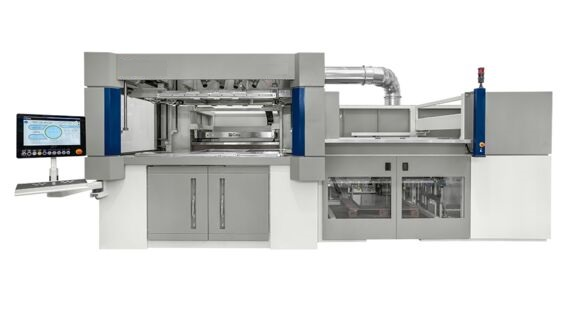
\includegraphics[width=\linewidth]{figures/thermoforming_machine.jpeg}
		\caption{Thermoforming machine}
		\label{fig:thermoforming_machine}
	\end{subfigure}
	\hspace{0.1\linewidth}
	\begin{subfigure}{0.35\linewidth}
		\centering
		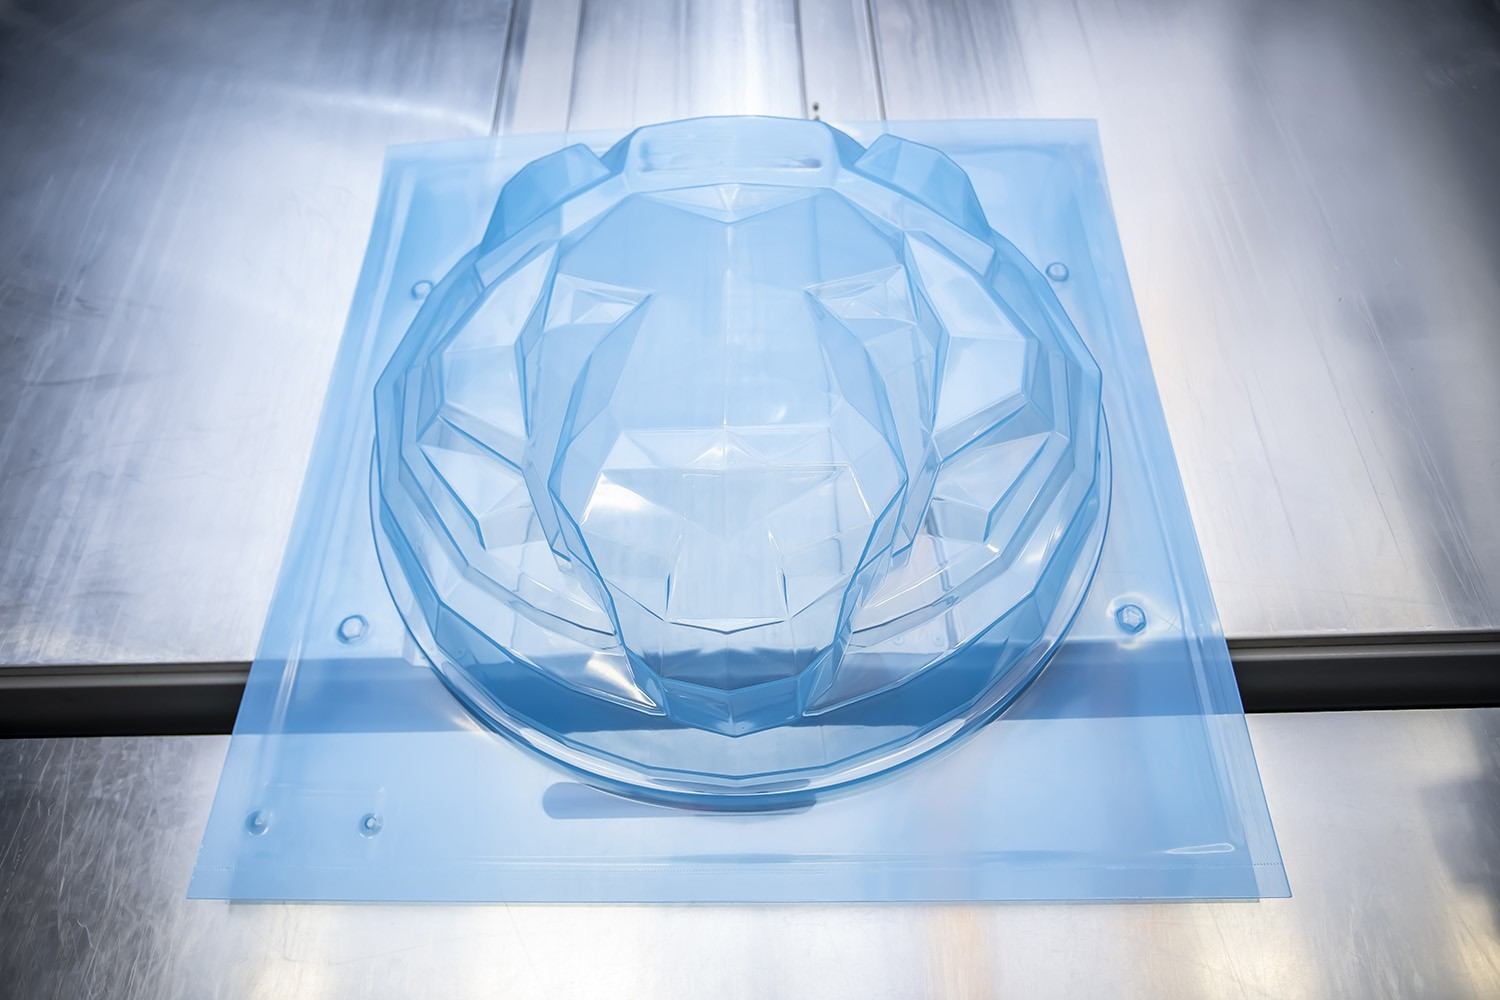
\includegraphics[width=\linewidth]{figures/thermoforming_result.jpg}
		\caption{Thermoformed product result}
		\label{fig:lion_shape}
	\end{subfigure}
	\caption{Thermoforming machine and an example of a thermoformed product obtained at the end of the process}
	\label{fig:thermoforming_combined}
\end{figure}

Given a specific mold geometry, such as the one shown in Figure~\ref{fig:lion_shape}, domain experts aim to apply greater heating to protruding regions of the sheet, which require increased flexibility, while limiting heating in other areas. Experts can therefore qualitatively define a desired core temperature distribution; however, achieving it typically requires multiple trial-and-error iterations to determine suitable machine parameters, resulting in significant time and material waste.

To address these challenges, we propose two artificial neural network (ANN) models. The first is a surrogate model of a physics-based simulator, designed to provide fast and accurate predictions of the temperature distribution at the core of the sheet. This surrogate model is then used to train a second network, an inverse model that predicts machine parameters from a desired temperature distribution while explicitly accounting for process cost.

Although the inverse model can reduce process costs, its predictions may deviate from the target temperature distribution due to the ill-posed nature of the inverse problem, in which different machine parameter configurations may produce similar temperature distributions. Reducing these deviations is important to improve the robustness of the model, which is trained on simulator-generated data and must be applied to real-world cases that may exhibit significant variability in product geometry and forming requirements.

To this end, a targeted optimization step is applied at the level of individual instances. This procedure refines the inverse model solution by reducing the temperature distribution error while adjusting the trade-off between thermal accuracy and process cost.

One of the main challenges in applying data-driven approaches in industrial settings is data scarcity. As noted by Wanigasekara et al.~\cite{wanigasekara2021machine}, thermoforming can be considered a small-data problem due to the high cost and time required for data acquisition. To address this limitation, we generated a dataset using a simulation tool provided by SCM Group S.p.A., which combines a physics-based simulator with a coupled machine control model. A total of \num{18432} samples were generated using \emph{Latin Hypercube Sampling} (LHS)~\cite{loh1996latin}, of which \num{16384} were used for training and 2~048 for validation. The test set consists of 45 real industrial cases collected by the industrial partner during one day of testing.

This study was conducted using an industrial thermoforming machine as reference, shown in Figure~\ref{fig:thermoforming_machine}, equipped with 240 halogen lamps arranged in two grids of 120 elements each, positioned above and below the sheet.

The remainder of this second part of the thesis is organized as follows. Chapter~\ref{chap:pt2_state_of_the_art} presents the state of the art; Chapter~\ref{chap:surrogate_model} presents the surrogate model; Chapter~\ref{chap:inverse_model} describes the inverse model; Chapter~\ref{chap:optimization} introduces the optimization strategy; and Chapter~\ref{chap:pt2_conclusion} concludes this part of the thesis.
